\chapter{Appendix Stuff}
\label{ch:appendix}

\begin{table}
\centering
\caption[XXX]{\textbf{XXX} \url{https://docs.google.com/spreadsheets/d/1eKuPU-XmqwrHkS_5-TgS8UnO5O-Hwe1kyRIpareywP4/edit?usp=sharing}}
\label{tab:studies}
\vspace*{5mm}
\begin{tabular}{ccc}
	\toprule
	{}  & TODO & TODO \\
	\midrule

	x & x & x\\
	x & x & x\\
	\bottomrule
\end{tabular}
\end{table}

\begin{table}
\centering
\caption[Network measures of studies]{\textbf{Network measures of studies} \url{https://docs.google.com/spreadsheets/d/1eKuPU-XmqwrHkS_5-TgS8UnO5O-Hwe1kyRIpareywP4/edit?usp=sharing}}
\label{tab:studies-measures}
\vspace*{5mm}
\begin{tabular}{ccc}
	\toprule
	{}  & TODO & TODO \\
	\midrule

	x & x & x\\
	x & x & x\\
	\bottomrule
\end{tabular}
\end{table}

\begin{table}
\centering
\caption[Network types of studies]{\textbf{Network types of studies} \url{https://docs.google.com/spreadsheets/d/1eKuPU-XmqwrHkS_5-TgS8UnO5O-Hwe1kyRIpareywP4/edit?usp=sharing}}
\label{tab:studies-nwtype}
\vspace*{5mm}
\begin{tabular}{ccc}
	\toprule
	{}  & TODO & TODO \\
	\midrule

	x & x & x\\
	x & x & x\\
	\bottomrule
\end{tabular}
\end{table}

\begin{figure}[htb]
	\centering
	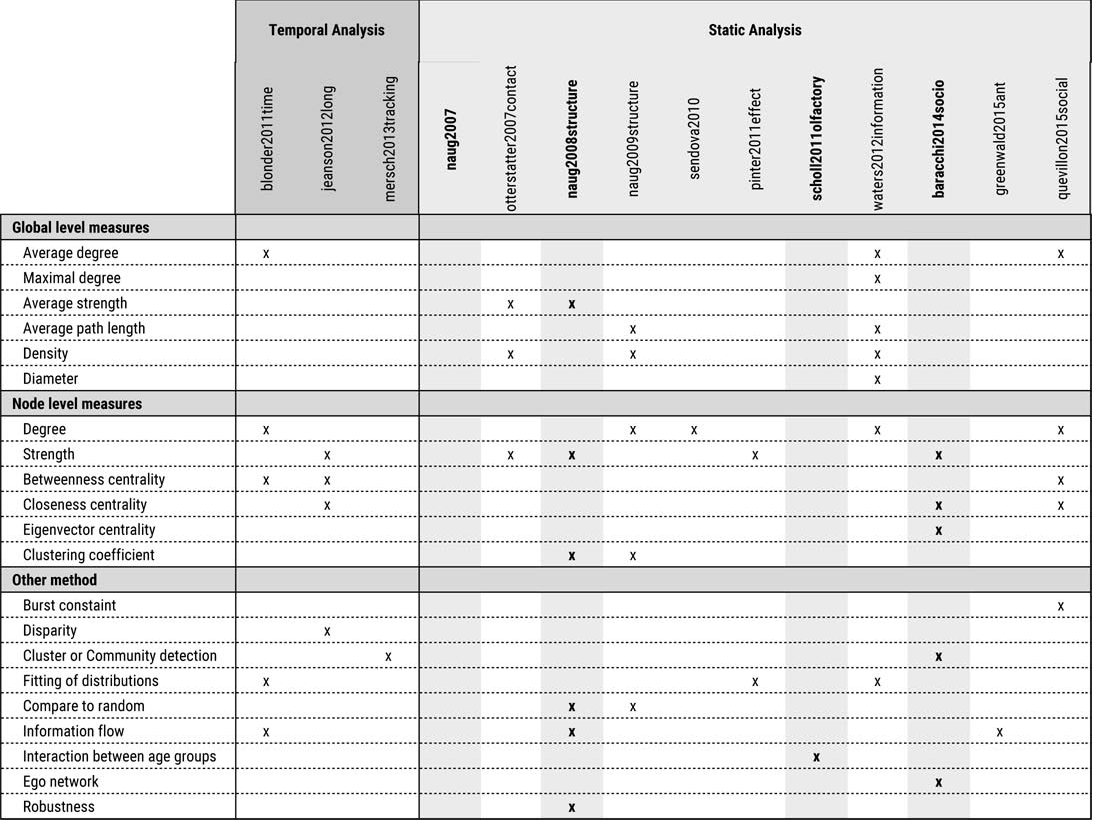
\includegraphics[width=1.0\textwidth]{Figures/study-measures}
	\caption[XXX]{\textbf{XXX} XXX}
	\label{fig:study-measures}
\end{figure}

\begin{figure}[htb]
	\centering
	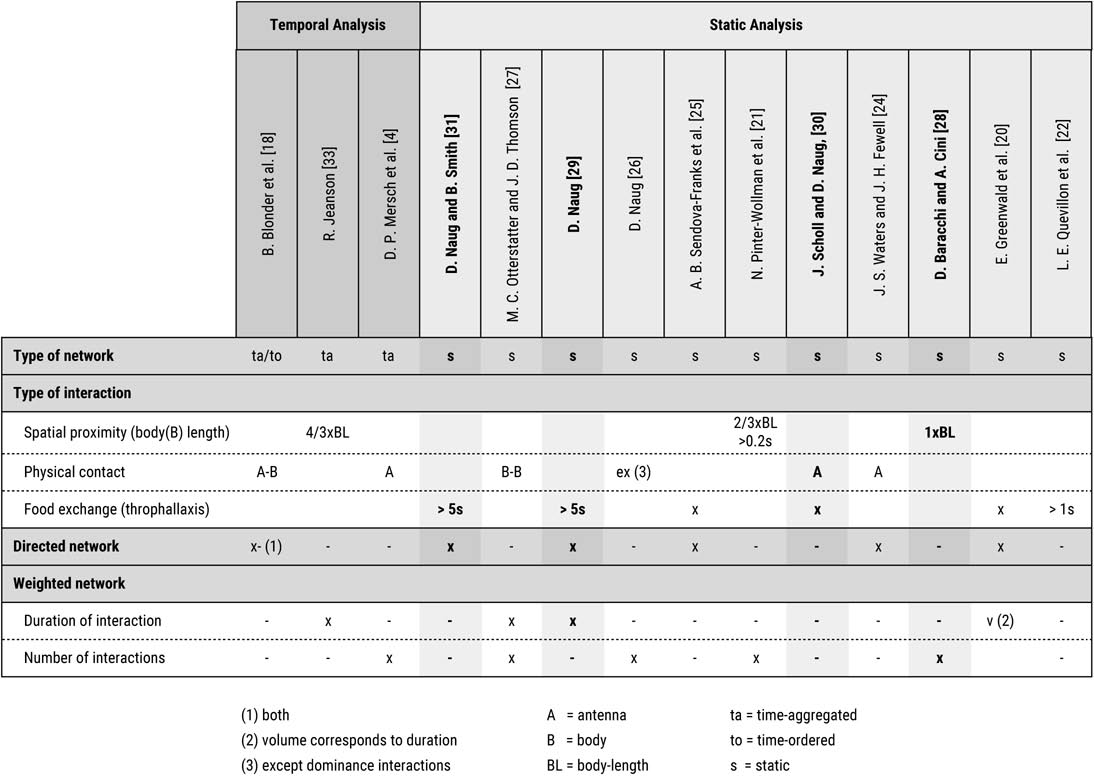
\includegraphics[width=1.0\textwidth]{Figures/study-nwtype}
	\caption[XXX]{\textbf{XXX} XXX}
	\label{fig:study-nwtype}
\end{figure}

\begin{figure}[htb]
	\centering
	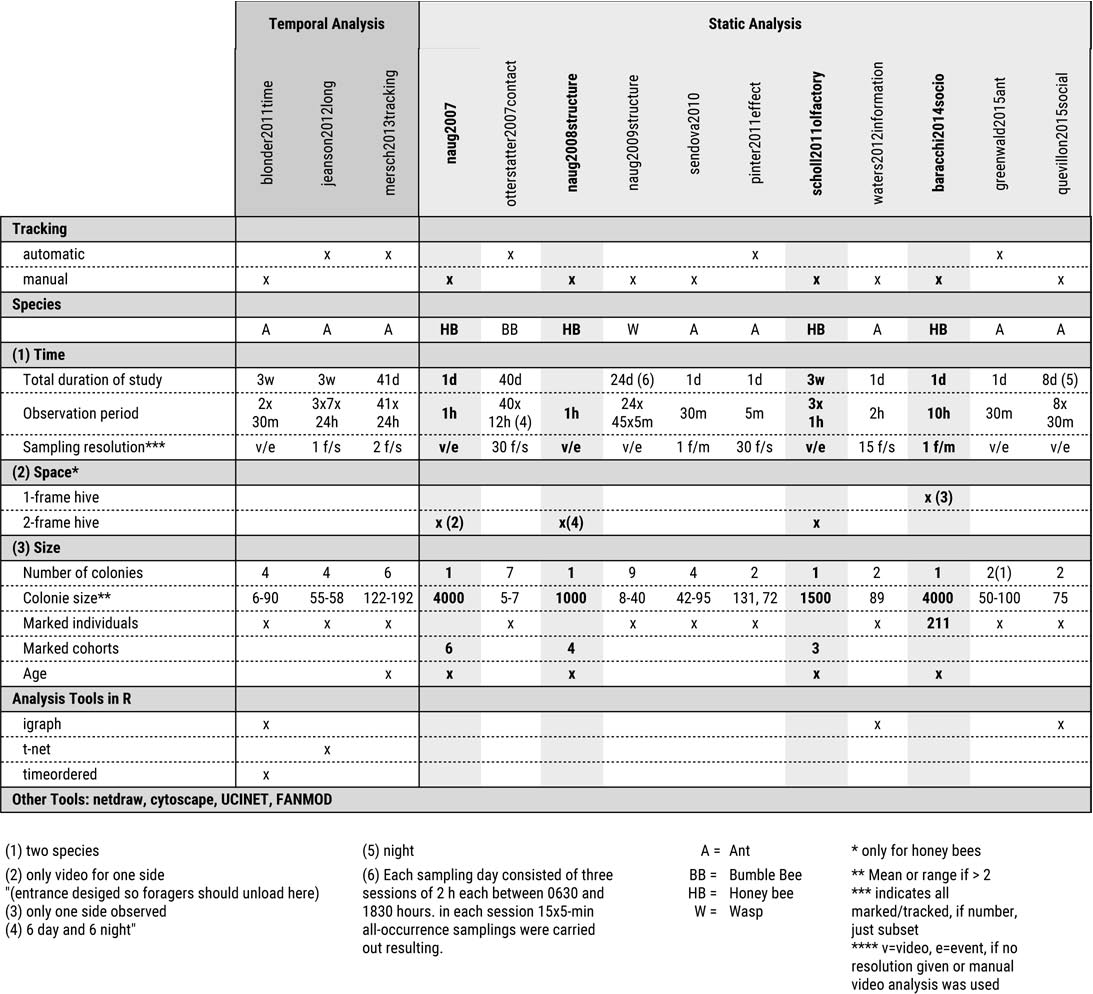
\includegraphics[width=1.0\textwidth]{Figures/study-study}
	\caption[XXX]{\textbf{XXX} XXX}
	\label{fig:study-study}
\end{figure}


\begin{figure}[htb]
	\centering
	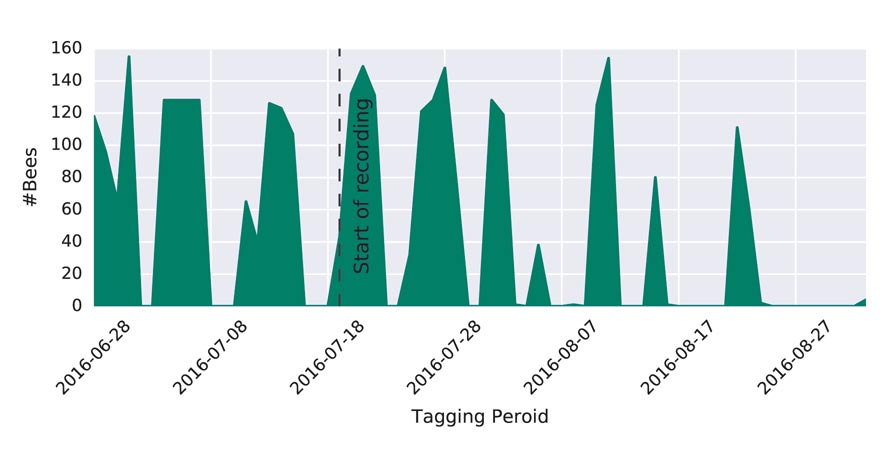
\includegraphics[width=1.0\textwidth]{Figures/tagging_period}
	\caption[Tagging frequency]{\textbf{Tagging frequency} The bees were primarily tagged during the week. On average 48 bees were tagged each day, considering only tagging days, the average is about 91. [TODO: combine with other image or make nicer!]}
	\label{fig:tagging-period}
\end{figure}

\begin{figure}[htb]
	\centering
	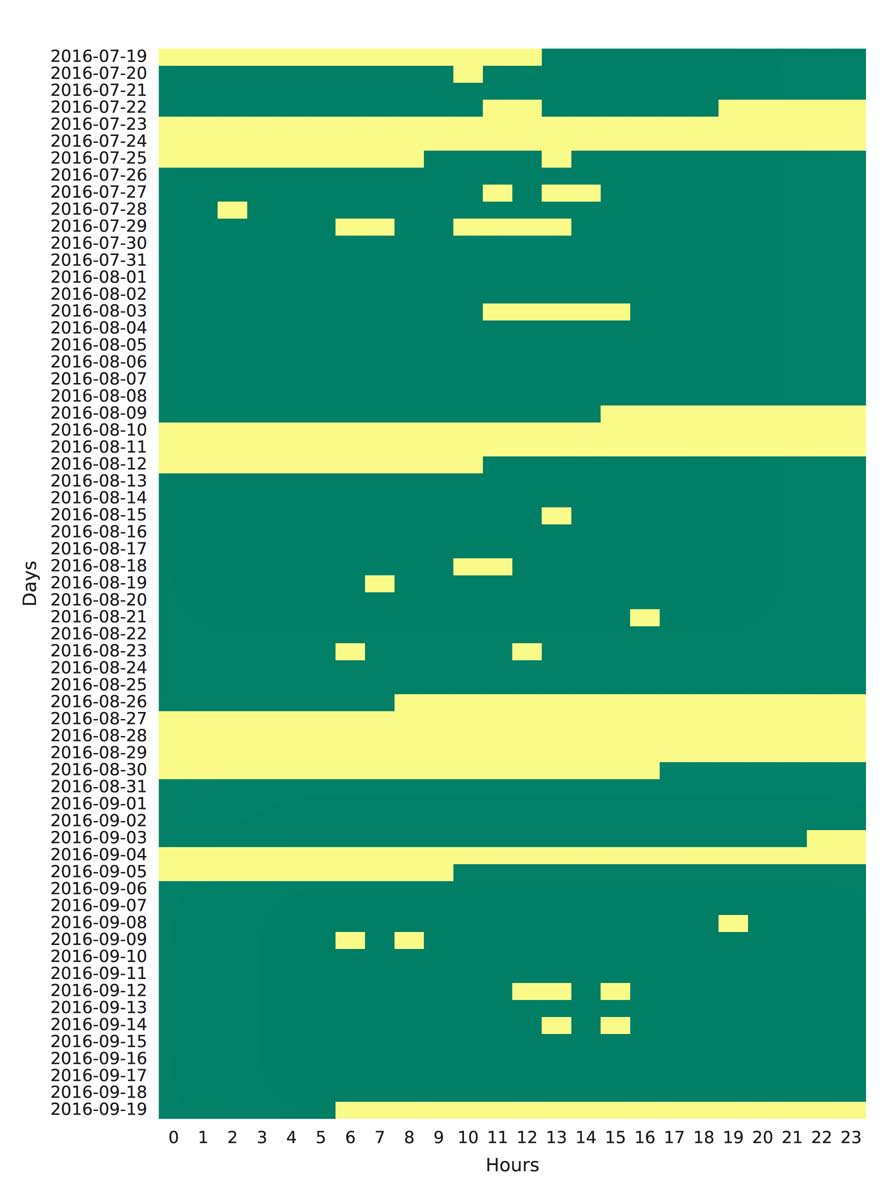
\includegraphics[width=1.0\textwidth]{Figures/recording}
	\caption[Recording season with maintainance and failures]{\textbf{Recording season with maintainance and failures} \emph{Green} indicates recording went without any big interruption; \emph{Yellow} indicates maintainance work or technical failures of one or all cameras. This is calculated using the expected number of files produced by each camera per hour. [TODO, reduzieren auf eine Info pro Tag (keine stuendliche aufloesung), kombinieren mit anzahl der getaggten bienen pro tag, und welchen Zeitraum hab ich nun verwendet], ausserdem Zeit von links nach rechts!, evtl. kein Datum, sonder Tage durchnummerieren}
	\label{fig:observation-period}
\end{figure}



\section{Network Analysis}
\label{app-analysis}

\begin{figure}[htb]
	\centering
	\begin{subfigure}[b]{1.0\textwidth}
		\centering
		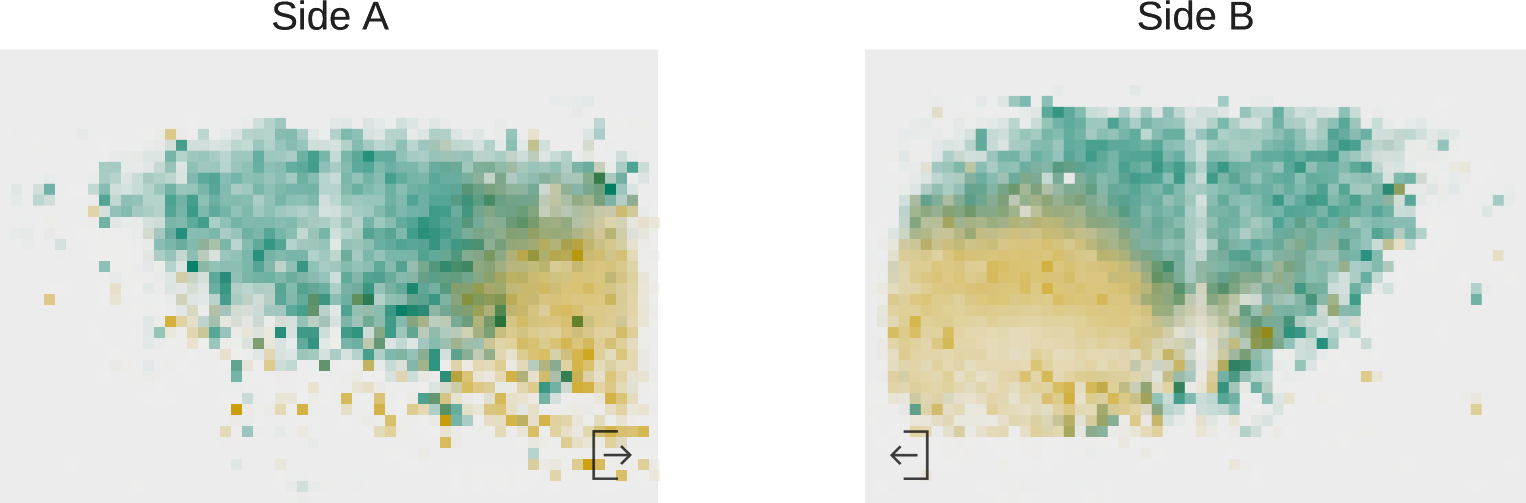
\includegraphics[width=\textwidth]{Figures/le_network1}
		\caption[Network 1]{Network 1}
		\label{fig:le1}
		\vspace*{5mm}
	\end{subfigure}
	%\vspace{1cm} 
	\begin{subfigure}[b]{1.0\textwidth}
		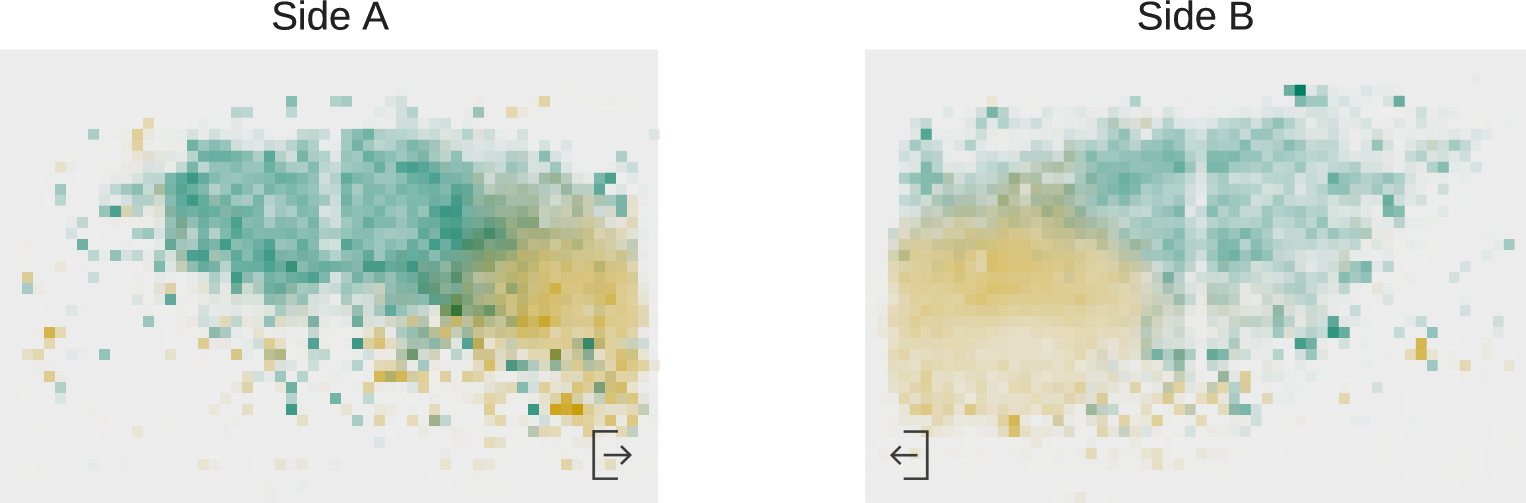
\includegraphics[width=\textwidth]{Figures/le_network2}
		\caption[Network 2]{Network 2}
		\label{fig:le2}
		\vspace*{5mm}
	\end{subfigure}
	%\vspace{1cm} 
	\begin{subfigure}[b]{1.0\textwidth}
		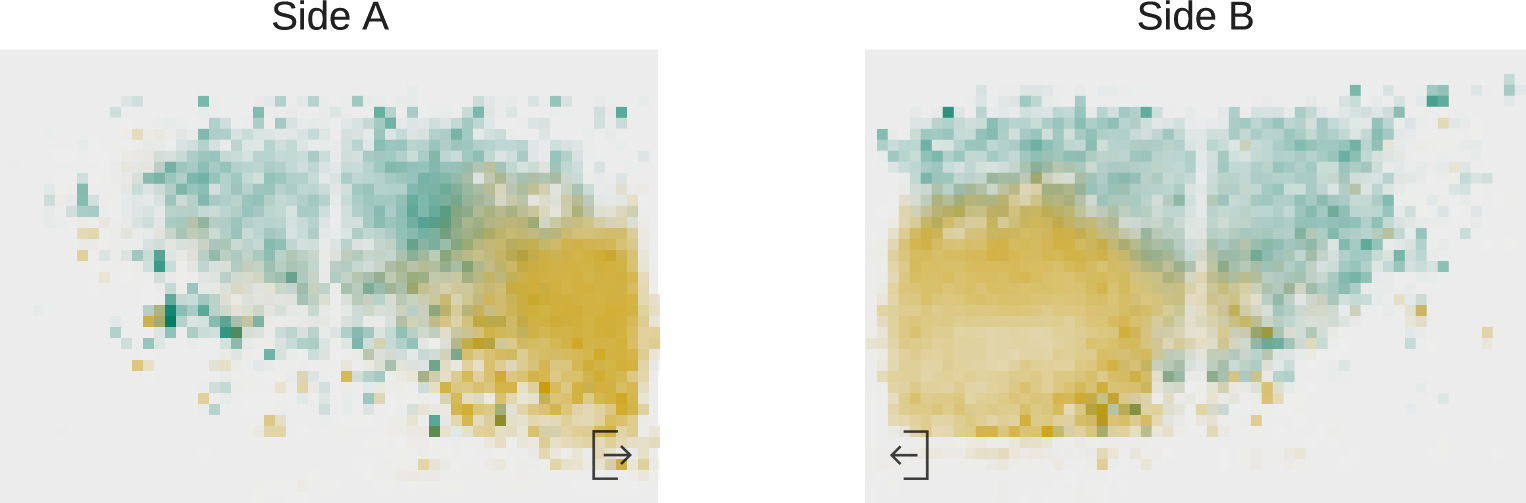
\includegraphics[width=\textwidth]{Figures/le_network3}
		\caption[Network 3]{Network 3}
		\label{fig:le3}
		\vspace*{5mm}
	\end{subfigure}
	\caption[Communities per network - leading eigenvector]{\textbf{Communities per network - leading eigenvector} The \emph{green} colour represents the younger community, containing the queen. The \emph{orange} color represents the older community. The hive exit on side A is on the bottom right and on side B on the bottom left. The data is aggredated for the complete timeframe of ten hours.}
	\label{fig:communitiesPerNetworkLE}
\end{figure}

\begin{figure}[htb]
	\centering
	\begin{subfigure}[b]{1.0\textwidth}
		\centering
		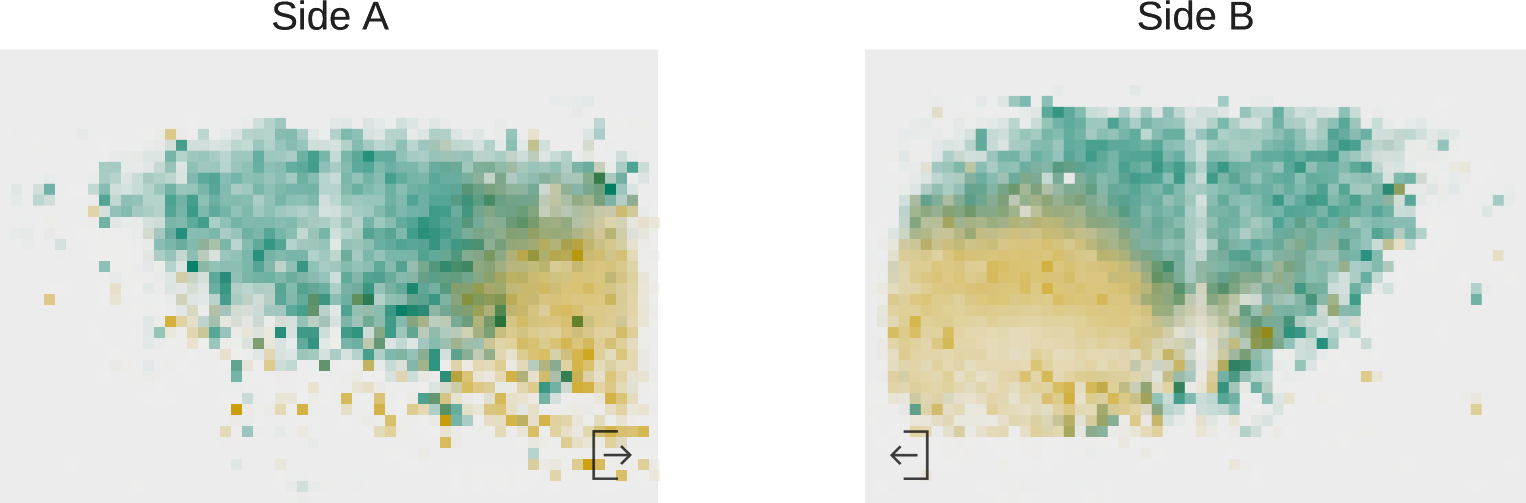
\includegraphics[width=\textwidth]{Figures/wt_network1}
		\caption[Network 1]{Network 1}
		\label{fig:wt1}
		\vspace*{5mm}
	\end{subfigure}
	%\vspace{1cm} 
	\begin{subfigure}[b]{1.0\textwidth}
		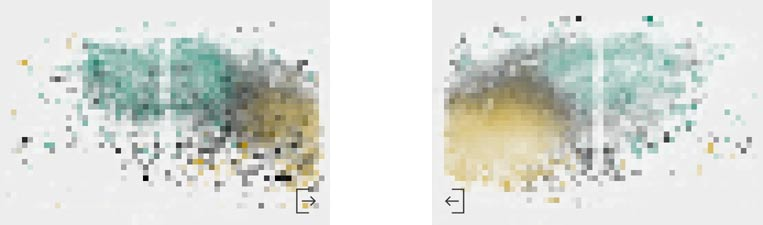
\includegraphics[width=\textwidth]{Figures/wt_network2}
		\caption[Network 2]{Network 2}
		\label{fig:wt2}
		\vspace*{5mm}
	\end{subfigure}
	%\vspace{1cm} 
	\begin{subfigure}[b]{1.0\textwidth}
		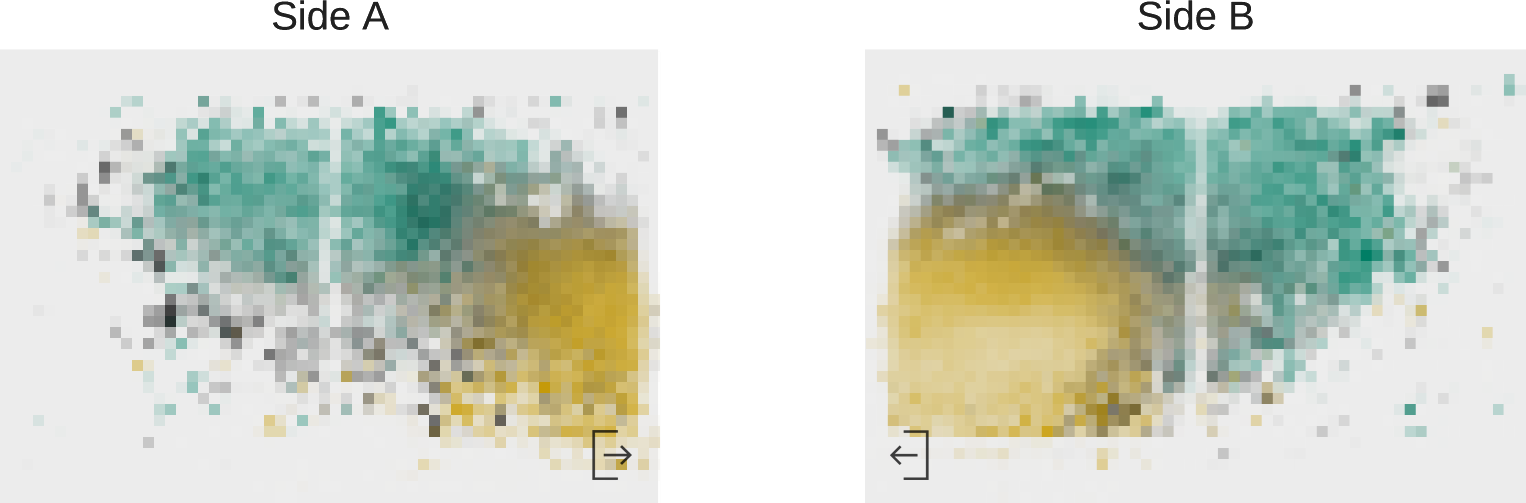
\includegraphics[width=\textwidth]{Figures/wt_network3}
		\caption[Network 3]{Network 3}
		\label{fig:wt3}
		\vspace*{5mm}
	\end{subfigure}
	\caption[Communities per network - walktrap]{\textbf{Communities per network - walktrap} The \emph{green} colour represents the younger community, containing the queen. The \emph{orange} color represents the older community. The \emph{gray} represents the middle-age community. The hive exit on side A is on the bottom right and on side B on the bottom left. The data is aggredated for the complete timeframe of ten hours.}
	\label{fig:communitiesPerNetworkWT}
\end{figure}

\begin{figure}[htb]
	\centering
	\begin{subfigure}[b]{1.0\textwidth}
		\centering
		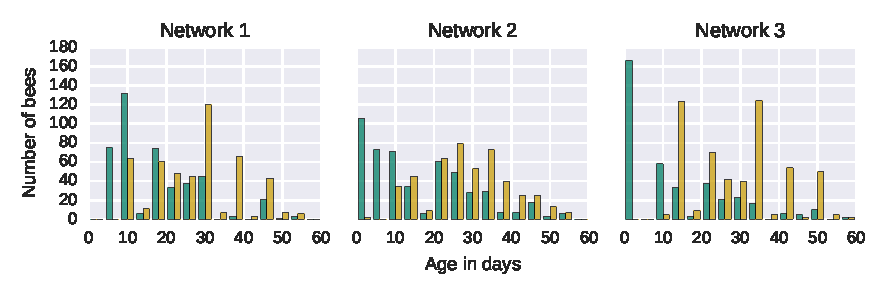
\includegraphics[width=1.0\textwidth]{Figures/ageDistribution-LE}
		\caption[Leading eigenvector]{Leading eigenvector}
		\label{fig:ageLE}
		\vspace*{5mm}
	\end{subfigure}
	%\vspace{1cm} 
	\begin{subfigure}[b]{1.0\textwidth}	
		\centering
		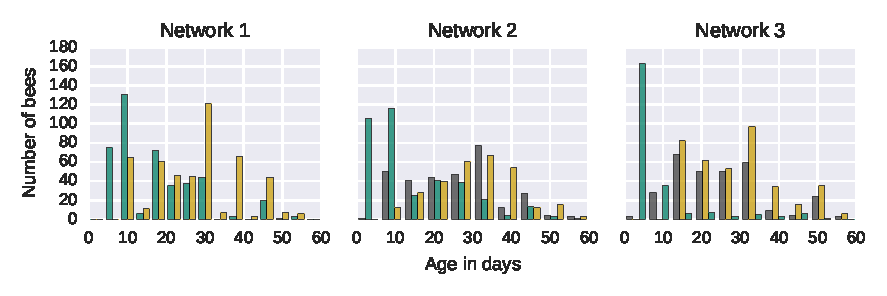
\includegraphics[width=1.0\textwidth]{Figures/ageDistribution-WT}
		\caption[Walktrap]{Walktrap}
		\label{fig:ageWT}
		\vspace*{5mm}
	\end{subfigure}
	%\vspace{1cm}
	\caption[Age distribution for each community and network] {\textbf{Age distribution for each community and network} The \emph{green} bar is the community containing the queen. The queens age is not included in the statistic. The \emph{orange} bars coresspond to the second community, containing older bees. The \emph{gray} bars is a third community only revealed by walktrap and contains middle-aged bees.}
	\label{fig:ageDistribution}
\end{figure}

\begin{figure}[!t]
	\centering
	\begin{subfigure}[b]{1.0\textwidth}
	\centering
	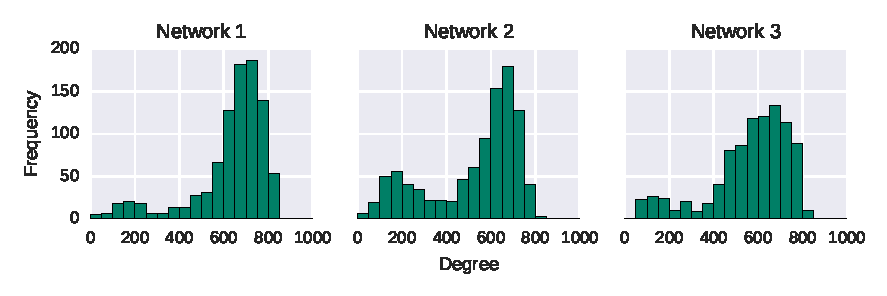
\includegraphics[width=0.92\textwidth]{Figures/stat-degreeDist}
	\caption[Degree distribution]{Degree distribution}
	\label{fig:statDegreeDist}
	\end{subfigure} 
	\begin{subfigure}[b]{1.0\textwidth}
	\centering
	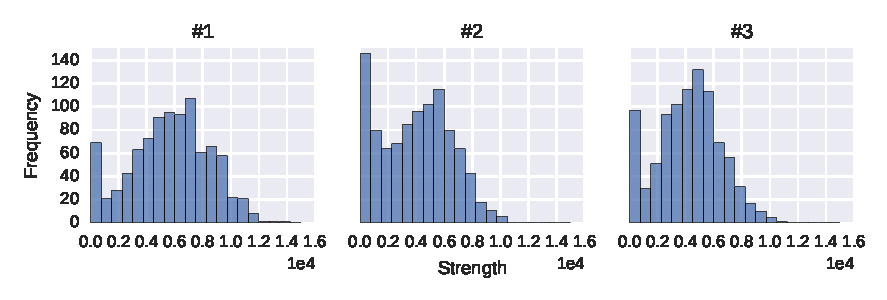
\includegraphics[width=0.92\textwidth]{Figures/stat-strengthDist}
	\caption[Strength distribution]{Strength distribution}
	\label{fig:statStrengthDist}
	\end{subfigure}
	\begin{subfigure}[b]{1.0\textwidth}
	\centering
	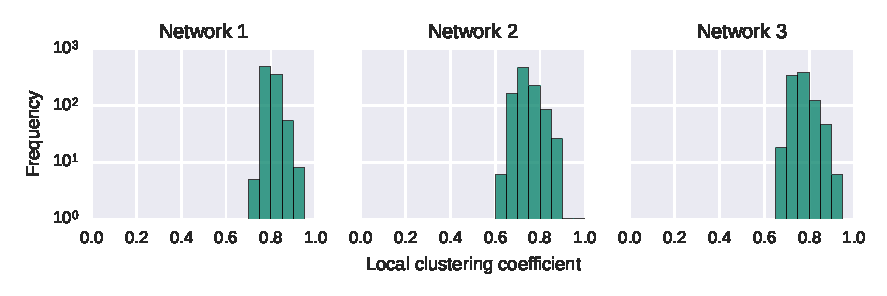
\includegraphics[width=0.92\textwidth]{Figures/stat-lccDist}
	\caption[Local clustering coefficient]{Local clustering coefficient}
	\label{fig:statlccDist}
	\end{subfigure}
	\begin{subfigure}[b]{1.0\textwidth}
	\centering
	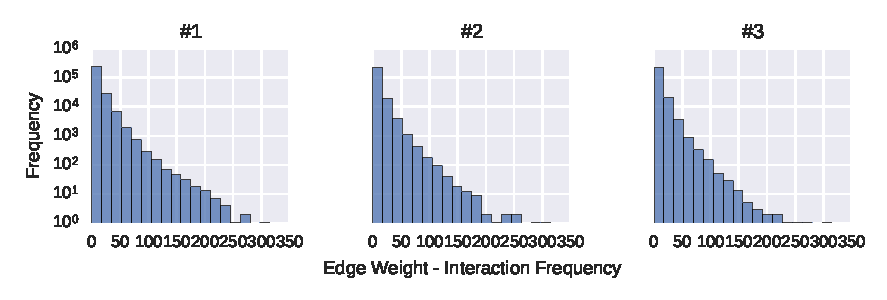
\includegraphics[width=0.92\textwidth]{Figures/stat-edgeWeightDist}
	\caption[Edge weight distribution]{Edge weight distribution}
	\label{fig:statEdgeWeightDist}
	\end{subfigure}
	\caption[Degree, strength and edge weight distribution]{\textbf{Degree, strength and edge weight distribution} for all three networks.}
	\label{fig:distributions}
\end{figure}

\begin{figure}[htb]
	\centering
	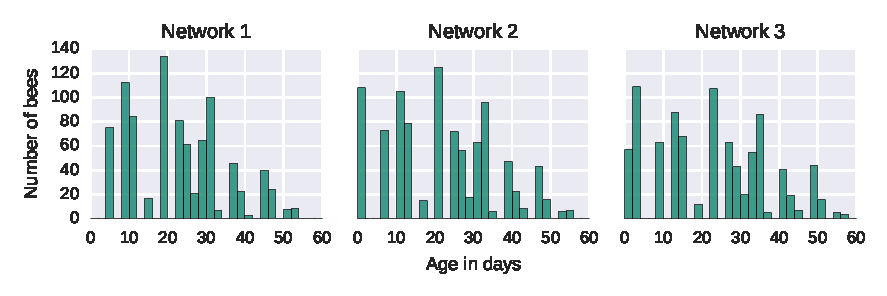
\includegraphics[width=1.0\textwidth]{Figures/ages}
	\caption[Age distribution per network]{\textbf{Age distribution per network} The width of a bar corresponds to two days. For each network bees with a negative age and the queen were removed (11, 10, and 9 bees).}
	\label{fig:ages}
\end{figure}